Un usuario contesta las preguntas debajo del cuestionario propuesto.

\subsection{Subpaso 1-A: Escala de dificultad}
Este paso aplica que  un usuario conteste la escala de dificultad de la pregunta propuesta. 
La escala va desde el 0 (muy fácil) hasta 10 ( Muy difícil) 
\begin{enumerate}
	\item Seleccione el número que corresponda a cada pregunta  en la escala de
	 dificultad
   
    \begin{figure}[hbtp]
	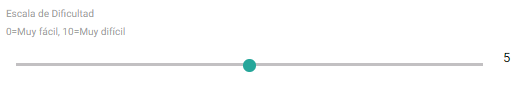
\includegraphics[scale=0.6]{images/Interfaz/IUGS-3escaladificultad.png}
	\caption{Escala de dificultad}
	\end{figure}
\end{enumerate}


\subsection{Subpaso 1-B: Opinión de la pregunta}
Este paso aplica si el usuario desea poner un comentario de cada una de las preguntas
\begin{enumerate}
	\item Presione \textbf{Opinión de la pregunta}
	\item Escriba su comentario
	\begin{figure}[hbtp]
	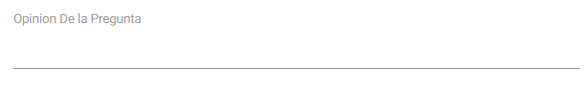
\includegraphics[scale=0.6]{images/Interfaz/IUGS-3opinionPregunta.png}
	\caption{Escala de dificultad}
	\end{figure}
\end{enumerate}